\title{\href{http://www.libpng.org/pub/png}{PNG (Portable
  Network Graphics)}~\cite{roelofs1999png}}

\maketitle
\tableofcontents

\section{\href{http://www.libpng.org/pub/png/book/}{Posibilities}}
\begin{itemize}
\item \href{https://en.wikipedia.org/wiki/Lossless_compression}{Fully
  lossless}.
\item Only
  \href{https://en.wikipedia.org/wiki/Raster_graphics}{raster} (not
  \href{https://en.wikipedia.org/wiki/Vector_graphics}{vectorized})
  images.
\item Better funtionality and performance than
  \href{https://en.wikipedia.org/wiki/GIF}{GIF (Graphics Interchange
    Format)}, that uses an patented implementation of the
  \mylink{LZW}{LZW} algorithm, and
  \href{https://en.wikipedia.org/wiki/TIFF}{TIFF (Tagged Image File
    Format)}.
\item Free usage and free from patents.
\item
  \href{https://en.wikipedia.org/wiki/Palette_(computing)}{Palletized
    images} (up to 256 colors), true color images (up to
  48-bits/pixel) and grayscale images (up to 16-bits/pixel).
\item On-the-fly encoding and decoding (streamability).
\item \href{https://en.wikipedia.org/wiki/Alpha_compositing}{Alpha
  channels} (variable transparency).
\item \href{https://en.wikipedia.org/wiki/Gamma_correction}{Gamma
  correction} (cross-platform control of image brightness).
\item
  \href{https://en.wikipedia.org/wiki/Progressive_scan}{Progressive}
  and
  \href{https://en.wikipedia.org/wiki/Interlacing_(bitmaps)}{interlazed}
  images.
\item
  \href{http://www.libpng.org/pub/png/book/chapter08.html#png.ch08.div.6}{Progressive
    reconstructions} by means of spatial scalability.
\end{itemize} 

\section{Codec}
\begin{center}
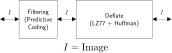
\includegraphics[width=20cm]{PNG_codec_ext}
\end{center}

\section{Filtering (encoding)}
\begin{itemize}
\item Optional.
\item Predictive encoder that reduces the spatial correlation.
\item Pixels are translated to prediction residues (errors):
  \begin{displaymath}
    E = X - \hat{X}
  \end{displaymath}
  where $X$ is the pixel-value and $\hat{X}$ its prediction.
\item The entropy of the residue image is typically smaller than in
  the original image, and the residues follow a
  \href{https://en.wikipedia.org/wiki/Laplace_distribution}{Lapace
    probability distribution}, centered in 0 (the average of the
  prediction error is 0).
\item Available predictors (``filters''):
  \begin{center}
    \begin{tabular}{cc}
      \begin{tabular}{rcl}
        Type & Predictor & Prediction \\
        \hline
        0 &	None 	& $\hat{X}\leftarrow 0$ \\
        1 &	Sub 	& $\hat{X}\leftarrow A$ \\
        2 &	Up 	& $\hat{X}\leftarrow B$ \\
        3 &	Average & $\hat{X}\leftarrow (A+B)/2$ \\
        4 &	Paeth 	& $\hat{X}\leftarrow A + B - C$
      \end{tabular}
      &
      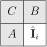
\includegraphics[width=3cm]{contexto_prediccion}
    \end{tabular}
  \end{center}
\item To increase the compression ratio (considering that the best
  predictor can depend on the area of the image that is being
  compressed), the predictor can be changed in the middle (of the
  encoding) of an image.
\end{itemize}

\section{``Deflate'' (encoding)}
\begin{itemize}
\item It's a generic text-compression algorithm based on
  \mylink{LZ77}{LZ77} and \mylink{Huffman_coding}{Huffman coding},
  written by
  \href{https://en.wikipedia.org/wiki/Jean-loup_Gailly}{Jean-loup
    Gailly} and \href{https://en.wikipedia.org/wiki/Mark_Adler}{Mark
    Adler}\footnote{Authors of The Data Compression Book
    \cite{Nelson96}}.
\item LZ77 removes the statistical \mylink{redudancy} of high order
  (remember that the preditor has removed the spatial redundancy).
\item The Huffman encoder removes the statistical redundancy of order
  0. The \mylink{probabilistic_models}{probabilistic model} used is
  adaptive and initially empty.
\end{itemize}


\section*{Let's go to the lab!}
\begin{itemize}
\item Use the \texttt{pnmtopng} command line tool to fill the table:
\begin{verbatim}
   Codec | lena boats pepers zelda Average
---------+--------------------------------
pnmtopng | 
\end{verbatim}
\end{itemize}

\bibliography{image-compression}
